\documentclass[11pt,reqno]{amsart}

\usepackage[T1]{fontenc}
\usepackage{lmodern}
\usepackage{amsmath,amssymb,mathtools}
\usepackage{graphicx}
\usepackage{xcolor}
\usepackage{microtype}
\usepackage[colorlinks=true,linkcolor=blue!55!black,citecolor=blue!55!black,urlcolor=blue!55!black]{hyperref}
\hypersetup{
  pdftitle={Positive-Parameter Two-End Spatial Dynamics in the Van der Pol Reaction-Diffusion System},
  pdfauthor={Haibo Lu},
  pdfkeywords={van der Pol reaction-diffusion system, reversible Hamiltonian spatial dynamics, saddle-focus homoclinic, singular exits, action finite parts, stationary patterns}
}

\graphicspath{{figures/}}
\numberwithin{equation}{section}

\newtheorem{theorem}{Theorem}[section]
\newtheorem{proposition}[theorem]{Proposition}
\newtheorem{lemma}[theorem]{Lemma}
\newtheorem{corollary}[theorem]{Corollary}
\theoremstyle{definition}
\newtheorem{hypothesis}[theorem]{Hypothesis}
\theoremstyle{remark}
\newtheorem{remark}[theorem]{Remark}

\newcommand{\R}{\mathbb R}
\newcommand{\cG}{\mathcal G}
\newcommand{\cH}{\mathcal H}
\newcommand{\cP}{\mathcal P}
\newcommand{\cR}{\mathcal R}
\newcommand{\cW}{\mathcal W}
\newcommand{\cA}{\mathcal A}
\newcommand{\Chi}{\operatorname{Chi}}
\newcommand{\Fix}{\operatorname{Fix}}
\newcommand{\spec}{\operatorname{spec}}
\newcommand{\norm}[1]{\left\lVert #1\right\rVert}
\newcommand{\dd}{\,d}

\title[Two-end spatial dynamics in van der Pol]{Positive-Parameter Two-End Spatial Dynamics in the Van der Pol Reaction--Diffusion System}
\author{Haibo Lu}
\date{August 28, 2026}

\subjclass[2020]{35B36, 35K57, 34C37, 34E15, 37J46}
\keywords{van der Pol reaction--diffusion system, reversible Hamiltonian spatial dynamics, saddle-focus homoclinic, singular exits, action finite parts, stationary patterns}

\begin{document}

\begin{abstract}
We study stationary solutions of the one-dimensional van der Pol
reaction--diffusion system in a singular positive-diffusion cusp.  Assuming a
frozen, publicly archived RFSN-II core and return--exit package, we prove on a
nonempty compact positive parameter annulus that the stationary spatial system
has an exhaustive high-winding first-return/first-exit relation.  The two
noncompact exits must be rebuilt from the full positive-parameter equations:
one is a finite-spatial-distance pole with a Laurent--logarithmic action finite
part, while the other is an infinite-distance algebraic end carried by a
normally expanding future-staying hypersurface.  We resolve the
$K_2\to K_1\to$ outer matching corner, prove reference-subtracted length and
action finite parts at the algebraic end, and attach both terminal potentials
to the exact branch cocycle.  The trapped return system is coded by a
two-vertex countable shift and yields spatially periodic, localized
multipulse, and bounded aperiodic stationary PDE profiles.  The result concerns
stationary spatial dynamics; it does not assert temporal stability, selection
from a Turing bifurcation, or canard identification.
\end{abstract}

\maketitle

\section{Problem, geometry, and conditional main result}\label{sec:intro}

\subsection{The physical stationary Hamiltonian}

Consider
\begin{equation}\label{eq:pde}
 \begin{aligned}
  u_t&=v-f(u)+d u_{\mathsf x\mathsf x},\\
  v_t&=\epsilon(a-u)+v_{\mathsf x\mathsf x},
  \qquad f(u)=\frac13u^3-u,
 \end{aligned}
 \qquad \mathsf x\in\R,
\end{equation}
where $d>0$ and $\epsilon>0$.  Its homogeneous state is
$(u,v)=(a,f(a))$.  Write $\delta=\sqrt d$ and introduce
\begin{equation}\label{eq:physical-spatial}
 \delta u_{\mathsf x}=p,\qquad
 \delta p_{\mathsf x}=f(u)-v,\qquad
 v_{\mathsf x}=q,\qquad
 q_{\mathsf x}=\epsilon(u-a).
\end{equation}
Stationary profiles of \eqref{eq:pde} are precisely the complete spatial
orbits of \eqref{eq:physical-spatial}.  With
\begin{equation}\label{eq:G-lambda}
 \begin{aligned}
  F(u)&=\frac1{12}u^4-\frac12u^2,\\
  \cG_\delta
  &=\frac12(\epsilon p^2-q^2)
    -\epsilon\{F(u)+(a-u)v\},\\
  \lambda_\delta&=\epsilon p\,du-\delta^{-1}q\,dv,
 \end{aligned}
\end{equation}
direct differentiation gives $d\cG_\delta/d\mathsf x=0$.  Moreover, if
$\omega_\delta=d\lambda_\delta$, then
\begin{equation}\label{eq:physical-Hamiltonian}
 \iota_{X_{\mathsf x}}\omega_\delta
   =dH_{\rm ph},\qquad
 H_{\rm ph}=-\frac{\cG_\delta-\cG_\delta(O)}{\delta},
 \qquad O=(a,0,f(a),0).
\end{equation}
The reverser
\begin{equation}\label{eq:reverser}
 \cR(u,p,v,q)=(u,-p,v,-q)
\end{equation}
is anti-symplectic.  Thus the zero-energy stationary spatial problem is a
reversible exact Hamiltonian system.  The sign and clock in
\eqref{eq:physical-Hamiltonian} matter for every action formula below.

The model and the singular Turing-canard regime were analyzed in
\cite{VoDoelmanKaper2025}.  We use its physical equations and blow-up charts,
but not a positive-parameter noncompact-end theorem: neither end used here is
obtained by ordinary persistence from the singular core.  The saddle-focus
homoclinic mechanism behind the return geometry is classical
\cite{Devaney1976,Lerman1991}; the issue addressed here is the full
positive-parameter attachment of that compact mechanism to two inequivalent
singular exits of \eqref{eq:physical-spatial}.

\subsection{The cusp and the two terminal geometries}

Fix
\begin{equation}\label{eq:fixed-epsilon-A}
 0<\epsilon_-<\epsilon_+<\infty,\qquad A>0,
\end{equation}
and parameterize the positive cusp by
\begin{equation}\label{eq:cusp}
 d=r^4,\qquad \delta=r^2,\qquad
 a=1+\sqrt\epsilon\,r^3a_2,\qquad |a_2|\le A.
\end{equation}
For small $r$, the homogeneous state is a saddle-focus for the spatial
system.  A source point that spends a long spatial time near this equilibrium
makes many rotations before meeting the global event block.  It may return
to the source, meet a finite auxiliary boundary, enter a pole at which
$u\to+\infty$ at a finite physical position, or enter an algebraic channel
that reaches $u=+\infty$ only as $\mathsf x\to+\infty$.

These last two outcomes are genuinely different.  At the pole, the physical
remaining distance $s=\mathsf x_{\rm b}-\mathsf x$ is the natural boundary
variable and the action requires a Laurent--logarithmic subtraction.  At the
algebraic end, $z=u^{-1}$ is the boundary defining function, physical length
diverges, and both length and action are normalized against a complete
reference tail.  The geometric relation is summarized in Figure~\ref{fig:geometry}.

\begin{figure}[t]
 \centering
 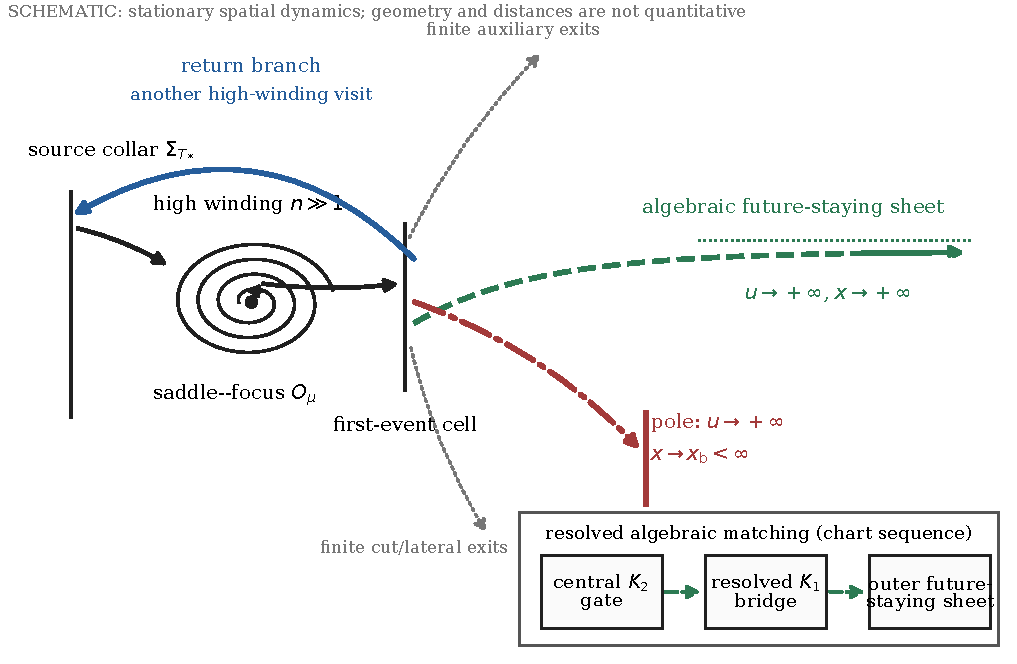
\includegraphics[width=\textwidth]{positive_two_end_geometry.pdf}
 \caption{Schematic stationary spatial geometry.  A point in the physical
 source collar makes a high-winding saddle-focus passage and then returns,
 reaches the finite-distance pole, reaches the infinite-distance algebraic
 end, or meets a named finite boundary.  The inset identifies the
 $K_2\to K_1\to$ outer bridge needed to attach the algebraic event.  Curve
 placement and distances are qualitative.  The figure does not represent
 temporal stability, Turing selection, or canard tracking.}
 \label{fig:geometry}
\end{figure}

\subsection{Frozen input}

The application theorem is conditional on a precisely delimited source
package.  This is preferable to hiding a computer-assisted core and a
fixed-system return theorem behind the phrase ``standard theory.''  The
immutable source, certificates, environment, and replay manifest are included
in the public release cited in \cite{LuRFSNII2026}; hashes and replay commands
are placed in the accompanying provenance supplement.

Throughout the paper, a mixed $C^k$ estimate is taken on the displayed fixed
state domains and means a uniform bound for all state/parameter derivatives
$D_Z^iD_\mu^j$ with $i+j\le k$ and $j\le2$.  Weighted saddle estimates may
also contain any fixed number of logarithmic derivatives
$D_{\log\nu}=\nu\partial_\nu$.

\begin{hypothesis}[Frozen RFSN-II package]\label{hyp:H}
The following data and analytic implication hold at the singular core and in
the associated fixed-system construction.
\begin{enumerate}
 \item[${\rm(H_{core})}$]
 The reversible exact Hamiltonian core
 \begin{equation}\label{eq:core}
  U'=P,\qquad P'=-U^2-V,\qquad V'=Q,\qquad Q'=U
 \end{equation}
 has the selected symmetric homoclinic orbit, transverse modulo the flow in
 the regular zero-energy hypersurface.  Its true unstable source graph and
 one compact physical event block have certified first-hit assignments,
 clean and neat incidences, exhaustive connected sign strata, fixed corner
 priorities, and strictly positive rank, speed, separation, and ordering
 margins.  The block contains distinct homoclinic, algebraic-directed, and
 pole-directed anchors.  Local uniqueness of the homoclinic is required only
 in the frozen shooting tube.  More specifically, on the nonempty pole phase
 interval $I_{\rm p}=[-0.2,0.2]$, put
 \[
  x=-U,\quad y=-P,\quad z_{\rm c}=-V,\quad\zeta=-Q,\quad
  D=\tfrac12x^2-z_{\rm c},\quad K=xy-\zeta .
 \]
 Every frozen source orbit in $I_{\rm p}$ has a strict first hit of $x=10$
 in $\{y>0,D>0,K>0\}$, with uniform positive hit-speed, cone-entry, and
 earlier-event margins.
 \item[${\rm(H_{Jost})}$]
 On a fixed central section $h_{\rm c}=0$, the singular comparison sheet has
 a defining function $g_{\rm a}$.  If
 $y_0(\phi,t)=\Phi_0^t(S_0(\phi))$ is the source flight to its selected
 intersection, then
 \begin{equation}\label{eq:source-incidence-core}
  s_0=dh_{\rm c}(F_0)(y_0)\ne0,\qquad
  \chi_0=Dg_{\rm a}(y_0)D_\phi y_0\ne0.
 \end{equation}
 The same sheet has an endpoint-normalized adjoint/Jost row $\psi$ and a
 fixed growing complement $\mathbf u_0$ whose directed exchange pairing is
 \begin{equation}\label{eq:exchange-core}
   \chi_{\rm ex}^0=\psi(\mathbf u_0)=144\sqrt3.
 \end{equation}
 \item[${\rm(H_{ret})}$]
 The frozen mixed-passage, selector, first-exit-family, covariance, and
 terminal-extension results are available with the following input--output
 contract.  Their inputs are: a compact $C^2$ family of reversible exact
 saddle-foci with an exact transverse-action passage; a transverse compact
 homoclinic transition with a fixed limiting matching rectangle, inverse and
 range margins; a finite state-$C^3$, parameter-$C^2$ clean physical event
 arrangement with strictly positive rank, speed, buffer, and ordering
 margins; and terminal potentials with one spare state derivative.  For
 \[
  T=-\alpha_\mu^{-1}\log|\nu|+t_{\mu,\sigma}+R_T,\qquad
  \Delta=-\frac{\beta_\mu}{\alpha_\mu}\log|\nu|
            +b_{\mu,\sigma}+R_\Delta,
 \]
 the remainders and their mixed two-jets are
 $O(|\nu|(1+|\log|\nu||))$ in $D_{\log\nu}$.  The event input includes every
 competing physical event and every pairwise event-time difference: an empty
 tie class has a positive gap, while a nonempty tie has nonzero conormal and
 a fixed priority.  Under these inputs the frozen results produce one uniform
 winding selector, completed contracting cross forms, the literal clean
 first-event census, exact section/gauge covariance, and the two-vertex
 countable terminal coding theorem with mixed two-jet estimates.
\end{enumerate}
\end{hypothesis}

Hypothesis~\ref{hyp:H} imports neither positive-parameter end.  The pole,
outer future-staying hypersurface, their matching, and both terminal finite
parts are all constructed below from \eqref{eq:physical-spatial}.  The
relative invariant-manifold statement used at the resolved $K_1$ corner and
the finite marked-atlas descent are proved in the companion proof archive,
using the classical compact invariant-manifold theory of
\cite{Fenichel1972,HirschPughShub1977} as boundaryless input.

\subsection{Main theorem}

\begin{theorem}[Conditional positive-parameter two-end theorem]\label{thm:main}
Assume Hypothesis~\ref{hyp:H}.  For the constants in
\eqref{eq:fixed-epsilon-A}, there exists $r_{\rm V}>0$ such that all of the
following statements hold uniformly on the nonempty compact positive annulus
\begin{equation}\label{eq:PV}
 \cP_{\rm V}=
 \left[\frac12r_{\rm V},r_{\rm V}\right]
 \times[-A,A]\times[\epsilon_-,\epsilon_+],
 \qquad \mu=(r,a_2,\epsilon),
\end{equation}
with physical parameters given by \eqref{eq:cusp}.

\begin{enumerate}
 \item The homogeneous state is a uniform saddle-focus, and the selected
 symmetric zero-energy homoclinic, its local stable and unstable manifolds,
 its exact local passage, and the compact central first-event block continue
 with two derivatives in $\mu$ in the blown-up parameter coordinates.

 \item There is a physical source collar $\Sigma_{T_*}$ and a finite
 compatible marked cover on which every sufficiently high-winding point has
 exactly one compact first event: return, stable cut, a named finite lateral
 event, or a terminal carrier labelled by the pole or algebraic outcome.
 Every point on either labelled terminal carrier has the stated subsequent
 noncompact future.  The connected strata form a literal
 disjoint census with no unnamed residual component.  For every sufficiently
 large local winding, both return target signs occur and the anchored pole
 and algebraic components are nonempty.  No nonemptiness is asserted for
 every other source sign or component label.  On chart overlaps, the physical
 first event agrees, while raw winding integers may differ by a bounded
 recoding.

 \item The pole occurs at a finite physical position
 $\mathsf x_{\rm b}$ and has a mixed-$C^2$ renormalized action
 \begin{equation}\label{eq:pole-main-fp}
 \cA^{\rm ren}_{\rm p}
  =\lim_{s\downarrow0}\left[
   \int_{\mathsf x_0}^{\mathsf x_{\rm b}-s}\lambda_\delta
   -2\epsilon\delta^3s^{-3}
   +2\epsilon\delta s^{-1}
   -\sqrt6\,\epsilon Z_0\log s\right].
 \end{equation}
 where $\mathsf x_0$ is the fixed source cut in the chosen marking; moving it
 changes the terminal potential by exactly the intervening finite branch
 action.
 The algebraic branch reaches $u=+\infty$ only at infinite physical distance.
 In the coordinate $Q=z^{-2}$ it has mixed-$C^2$ renormalized length and
 action
 \begin{equation}\label{eq:alg-main-fp}
  \begin{aligned}
   L^{\rm ren}_{\rm a}
    &=\lim_{Q\to\infty}
      \{L_{\mathrm{source}\to Q}-C_{\mathsf x,\mu}(Q)\},\\
   \cA^{\rm ren}_{\rm a}
    &=\lim_{Q\to\infty}
      \left\{\int_{\mathrm{source}\to Q}\lambda_\delta
                    -C_{\mathsf A,\mu}(Q)\right\},
  \end{aligned}
 \end{equation}
 where the counterterms are complete reference-tail integrals and satisfy
 \begin{equation}\label{eq:alg-counter-leading}
  \begin{aligned}
   C_{\mathsf x,\mu}(Q)
    &=q_*^{-1}Q^{1/2}+O_{C^2_\mu}(\log Q),\\
   C_{\mathsf A,\mu}(Q)
    &=-\frac{q_*}{5\delta}Q^{5/2}+O_{C^2_\mu}(Q^2),
    \qquad q_*=\sqrt{\epsilon/2}.
  \end{aligned}
 \end{equation}
 All finite branch actions and the two terminal potentials obey exact
 first-hit composition; closed actions are independent of admissible cuts,
 exact gauges, event-free section slides, and the local marking.

 \item In every marking, the trapped return set is conjugate to the
 two-vertex countable edge shift with edges
 \begin{equation}\label{eq:edges}
  (\sigma,n,\sigma'),\qquad \sigma,\sigma'\in\{+,-\},
  \qquad n\ge N.
 \end{equation}
 Primitive periodic words yield smooth spatially periodic stationary
 solutions of \eqref{eq:pde}; nonperiodic bi-infinite words yield bounded
 nonperiodic stationary solutions; and arbitrary finite admissible edge
 words with the
 selected unstable and stable endpoints yield homoclinic multipulse profiles
 converging to $(a,f(a))$ as $\mathsf x\to\pm\infty$.
\end{enumerate}
\end{theorem}

The set \eqref{eq:PV} is existential.  It is not the currently proposed
numerical box, and the theorem does not claim uniformity down to the cusp tip
$r=0$.  The parameter image in $(d,a,\epsilon)$ is a cusp, not a rectangular
box.

For completeness, the quantitative high-winding consequence is stated next.
Let
\begin{equation}\label{eq:alpha-beta}
 c_\mu=2ra_2+\sqrt\epsilon\,r^4a_2^2,\qquad
 \alpha_\mu=\frac12\sqrt{2+c_\mu},\qquad
 \beta_\mu=\frac12\sqrt{2-c_\mu}.
\end{equation}
For any
\begin{equation}\label{eq:kappa}
 0<\varkappa<\inf_{\mu\in\cP_{\rm V}}
                  \frac{2\pi\alpha_\mu}{\beta_\mu},
\end{equation}
the marked cover and $N$ may be chosen so that its cross forms and branch
potentials converge in mixed $C^2$ at rate
$C(1+n)^3e^{-\varkappa n}$.  In particular, for a fixed primitive cyclic
word with windings $n_0,\ldots,n_{m-1}$,
\begin{equation}\label{eq:period-asymptotic}
 L(\gamma_{\mathbf n})
 =\frac{2\pi r}{\epsilon^{1/4}\beta_\mu}
    \sum_{j=0}^{m-1}n_j
  +\mathcal L_{\boldsymbol\sigma,\mu}
  +O\!\left(\max_j(1+n_j)^3e^{-\varkappa n_j}\right),
\end{equation}
while its closed action has a finite marking-independent limit with the same
error.  The estimate is for fixed word length; it is not uniform when the
number of composed branches tends to infinity.  Here
$\boldsymbol\sigma$ denotes the cyclic sequence of source and target signs of
the fixed word, so the finite offset need not be a function of a single sign.

\subsection{Why the proof is not ordinary persistence}

The frozen theory reaches the compact central gates.  It does not identify
their positive-parameter futures.  The proof therefore has the following
causal spine:
\begin{equation}\label{eq:proof-spine}
\begin{gathered}
 \text{physical Hamiltonian and frozen core}
 \longrightarrow \text{central continuation},\\
 \text{pole-directed gate}
 \longrightarrow \text{positive pole and its finite part},\\
 \text{positive outer field}
 \longrightarrow \text{future-staying sheet},\\
 \text{central gate}+\text{outer sheet}+{\rm(H_{Jost})}
 \longrightarrow K_2\to K_1\to\text{outer matching},\\
 \text{matched sheet}
 \longrightarrow \text{algebraic length/action finite parts},\\
 \text{compact event block}+\text{two actual terminals}+{\rm(H_{ret})}\\
 \longrightarrow \text{physical first-event relation}
 \longrightarrow \text{stationary PDE profiles}.
\end{gathered}
\end{equation}
The pole changes dominant balance when $\delta>0$.  The algebraic branch
enters an outer slow regime and must be matched across a nonhyperbolic chart
corner.  These are the two obstructions removed in Sections~\ref{sec:pole}
and \ref{sec:outer}; Section~\ref{sec:coding} then performs only the minimal
replacement of the two finite gates by the actual terminals.

\section{Central continuation and the finite-distance pole}\label{sec:pole}

\subsection{Exact central scaling}

The cusp scaling is fixed before applying the imported core.  Put
\begin{equation}\label{eq:central-change}
 \begin{aligned}
  u&=a-\sqrt\epsilon\,r^2U,&
  p&=-\epsilon^{3/4}r^3P,\\
  v&=f(a)-\epsilon r^4V,&
  q&=-\epsilon^{5/4}r^3Q,&
  \xi&=\epsilon^{1/4}\mathsf x/r.
 \end{aligned}
\end{equation}
This sends the homogeneous state to the origin.  Direct substitution, with no
remainder, gives
\begin{equation}\label{eq:central-field}
 \begin{aligned}
  U'&=P,\\
  P'&=c_\mu U-V-(1+\sqrt\epsilon\,r^3a_2)U^2
       +\frac{\sqrt\epsilon}{3}r^2U^3,\\
  V'&=Q,\qquad Q'=U,
 \end{aligned}
\end{equation}
where the prime denotes $d/d\xi$ and $c_\mu$ is defined in
\eqref{eq:alpha-beta}.  The parameter-independent primitive and shifted
Hamiltonian are
\begin{equation}\label{eq:central-H}
 \begin{aligned}
  \lambda&=P\,dU-Q\,dV,\\
  \widehat H_\mu
  &=\frac12(Q^2-P^2)-UV+\frac{c_\mu}{2}U^2
   -\frac{1+\sqrt\epsilon r^3a_2}{3}U^3
   +\frac{\sqrt\epsilon}{12}r^2U^4,\\
  \iota_{F_\mu}d\lambda&=d\widehat H_\mu.
 \end{aligned}
\end{equation}
The exact physical conversions are
\begin{equation}\label{eq:clock-action-scales}
 d\mathsf x=r\epsilon^{-1/4}\,d\xi,\qquad
 \lambda_\delta=\epsilon^{9/4}r^5\lambda,\qquad
 H_{\rm ph}=\epsilon^{5/2}r^4\widehat H_\mu.
\end{equation}
At $r=0$, \eqref{eq:central-field} is exactly \eqref{eq:core}.  Its
characteristic polynomial at the origin is
$\zeta^4-c_\mu\zeta^2+1$, and hence its spectrum is
$\{\pm\alpha_\mu\pm i\beta_\mu\}$.

\begin{proposition}[Central continuation]\label{prop:central}
Under ${\rm(H_{core})}$ and the mixed-passage clause of
${\rm(H_{ret})}$, after decreasing the upper $r$-radius, the origin,
the selected symmetric homoclinic, and the compact central first-event block
continue on the closed blown-up parameter wedge.  The local invariant
manifolds and the homoclinic have two parameter derivatives with uniform
exponential tails.  A finite parameter cover carries reversible exact saddle
coordinates.  If $\nu$ is the signed transverse action, the passage time and
Kato-oriented phase satisfy
\begin{equation}\label{eq:passage}
 \begin{aligned}
  T_{\mu,\sigma}(\nu)
   &=-\alpha_\mu^{-1}\log|\nu|+t_{\mu,\sigma}
      +O_{\rm wl}(|\nu|),\\
  \Delta_{\mu,\sigma}(\nu)
   &=-\frac{\beta_\mu}{\alpha_\mu}\log|\nu|
      +b_{\mu,\sigma}+O_{\rm wl}(|\nu|),
 \end{aligned}
\end{equation}
where $O_{\rm wl}(|\nu|)$ denotes
$O(|\nu|(1+|\log|\nu||))$ after any two parameter derivatives and any fixed
number of logarithmic derivatives $\nu\partial_\nu$.  The continued event
block remains clean, neat, componentwise exhaustive, and separated by
uniform positive physical first-hit margins.
\end{proposition}

\begin{proof}
On fixed compact state sets, \eqref{eq:central-field} is a smooth $C^2$
parameter family converging to \eqref{eq:core}.  The saddle-focus rates stay
uniformly away from zero.  Parameter-dependent graph transforms give fixed
domain stable and unstable graphs; their Lyapunov--Perron equations may be
differentiated twice because the exponential dichotomy is uniform.  In a
weighted full-line space, the reversible matching equation for the selected
core orbit has invertible derivative by the certified transversality in
${\rm(H_{core})}$.  The implicit-function theorem therefore gives the
homoclinic and its two-derivative exponential tails.

The exact local passage follows from the reversible analytic saddle normal
form in ${\rm(H_{ret})}$ after tangent normalization to one Kato-transported
oriented spectral frame.  Direct normal-form quadrature on the radial
sections fixes the minus sign in the phase law in \eqref{eq:passage}; the
transverse action itself is unchanged.  Finally, all compact first-hit
speeds, active conormal ranks, empty incidences, earlier-event exclusions,
and ordering inequalities in ${\rm(H_{core})}$ are strict on compact sets.
Smooth first-hit dependence and a boundary-preserving controlled isotopy
retain the complete labelled incidence complex.  This proves the proposition.
\end{proof}

The two end labels in Proposition~\ref{prop:central} are still finite gates.
Nothing in compact first-hit stability implies that an orbit subsequently
reaches a noncompact end.

\subsection{Invariant cone and finite physical blow-up}

For the pole-directed branch write
\begin{equation}\label{eq:pole-central-vars}
 x=-U,\qquad y=-P,\qquad z=-V,\qquad \zeta=-Q,
\end{equation}
and set
\begin{equation}\label{eq:pole-cone}
 D=\frac12x^2-z,\qquad K=xy-\zeta,\qquad
 \mathcal K_\mu=\{x\ge10,\ y>0,\ D\ge0,\ K\ge0\}.
\end{equation}
The exact field gives
\begin{equation}\label{eq:pole-cone-identities}
 \begin{aligned}
  x'&=y,& D'&=K,\\
  y'&=D+(B-\tfrac12)x^2+c_\mu x+bx^3,&
  K'&=y^2+xy'-x.
 \end{aligned}
\end{equation}
where $B=1+\sqrt\epsilon r^3a_2$ and
$b=\sqrt\epsilon r^2/3>0$.  On the final small positive annulus,
$B\ge3/4$ and $|c_\mu|\le1$.  Hence the faces of
$\mathcal K_\mu$ point inward and, for $x\ge10$,
\begin{equation}\label{eq:pole-growth}
 y'>0,\qquad K'>0,\qquad
 y\frac{dy}{dx}\ge bx^3.
\end{equation}
The certified core source window has a strict first hit of $x=10$ in the
interior of this cone.  Proposition~\ref{prop:central} and a short event-free
flowbox slide retain that literal first hit for positive parameters.  From
\eqref{eq:pole-growth},
\begin{equation}\label{eq:pole-finite-time}
 y(x)^2\ge y(10)^2+\frac b2(x^4-10^4),\qquad
 \xi_{\rm b}-\xi=\int_x^\infty\frac{dX}{y(X)}<\infty.
\end{equation}
Thus the pole is reached in finite central and physical spatial time.
On the zero-energy level the exact identity is
\begin{equation}\label{eq:pole-energy-identity}
 y^2=\zeta^2-2xz+c_\mu x^2+\frac{2B}{3}x^3+\frac b2x^4.
\end{equation}
The lower bound in \eqref{eq:pole-finite-time} gives
\[
 \frac{d\zeta}{dx}=\frac{x}{y}=O(x^{-1}),\qquad
 \frac{dz}{dx}=\frac{\zeta}{y}=O((1+\log x)x^{-2}).
\]
Hence $z\to z_\infty$, $\zeta=O(1+\log x)$, and
\eqref{eq:pole-energy-identity} closes the uniform limits
\begin{equation}\label{eq:pole-central-sharp}
 \frac{y}{x^2}\to\sqrt{b/2},\qquad
 \zeta-\sqrt{2/b}\log x\to\zeta_\infty,\qquad
 z_\infty-z=O((1+\log x)x^{-1}).
\end{equation}
One further integration of $dx/d\xi=y$ and the exact physical inverse of
\eqref{eq:central-change} give the balance below.  In particular, the two
end labels range in a compact set on the transported source window.

\subsection{Regular-singular compactification and pole action}

Let $s=\mathsf x_{\rm b}-\mathsf x$ and $\ell=\sqrt6\,\delta$.  The sharp
balance obtained from the conserved energy and \eqref{eq:pole-growth} is
\begin{equation}\label{eq:pole-balance}
 \frac{su}{\ell}\to1,\qquad
 \frac{s^2p}{\ell\delta}\to1,\qquad
 q+\ell\epsilon\log s\to W_0,\qquad
 v-\ell\epsilon s\log s\to Z_0.
\end{equation}
Define
\begin{equation}\label{eq:pole-compact-vars}
 X=su/\ell,\qquad Y=s^2p/(\ell\delta),\qquad
 W=q+\ell\epsilon\log s,\qquad
 Z=v-\ell\epsilon s\log s,
\end{equation}
and use $\dot{}=s\,d/d\mathsf x$.  Substitution in
\eqref{eq:physical-spatial} gives the exact $C^3$ regular-singular field
\begin{equation}\label{eq:pole-compact-field}
 \begin{aligned}
  \dot s&=-s,& \dot X&=-X+Y,\\
  \dot Y&=-2Y+2X^3-s^2\delta^{-2}X
       -s^3(\ell\delta^2)^{-1}Z
       -\epsilon\delta^{-2}s^4\log s,\\
  \dot W&=\ell\epsilon(X-1)-a\epsilon s,&
  \dot Z&=s(W+\ell\epsilon).
 \end{aligned}
\end{equation}
At $s=0$ it has the two-dimensional equilibrium manifold
$X=Y=1$, parameterized by $(Z_0,W_0)$.  Its normal spectrum is
$\{-1,-4,+1\}$, while the two label directions have eigenvalue zero.  The
stable pole family therefore has normalized power spectrum
\begin{equation}\label{eq:pole-spectrum}
 \{-1,0,0,1,4\}.
\end{equation}

\begin{proposition}[Positive pole terminal]\label{prop:pole}
Under Hypothesis~\ref{hyp:H}, on a nonempty compact positive subannulus, the
transported pole source window
enters an open pole basin and reaches $u=+\infty$ at a finite physical
position.  Each pole orbit has unique labels $(Z_0,W_0,c_4)$ and a
polyhomogeneous expansion with admissible powers $1$ and $4$, including the
forced $s\log s$ and $s^4(\log s)^2$ terms.  On the fixed zero-energy level,
$c_4$ is determined uniquely because
\begin{equation}\label{eq:energy-c4}
 \partial_{c_4}\cG_\delta=-30\epsilon\delta^4\ne0.
\end{equation}
The action finite part \eqref{eq:pole-main-fp} exists with two mixed parameter
derivatives and satisfies exact moving-cut additivity.
\end{proposition}

\begin{proof}
Normal hyperbolicity of the compact label rectangles in
\eqref{eq:pole-compact-field} gives a four-dimensional local stable set: two
label directions and two stable fibers.  The uniform limits
\eqref{eq:pole-balance} and \eqref{eq:pole-central-sharp} show that every
transported source orbit converges to the interior of one common compact
label rectangle.  The defining staying-set characterization of the local
stable manifold therefore puts the entire window in that stable set.
Eliminating $Y$ yields
the scalar Fuchsian equation
\begin{equation}\label{eq:Fuchsian}
 (s\partial_s-4)(s\partial_s+1)(X-1)
 =6(X-1)^2+2(X-1)^3
  -\frac{s^2}{\delta^2}X-\frac{s^3}{\ell\delta^2}Z
  -\frac{\epsilon}{\delta^2}s^4\log s.
\end{equation}
The nonresonant powers two and three are forced; at the indicial root four,
the constant and logarithmic forcing produces
$s^4\log s$ and $s^4(\log s)^2$, with $c_4s^4$ the free stable mode.  The
Green inverse of $(s\partial_s-4)(s\partial_s+1)$ is bounded on the conormal
weight $s^5(1+|\log s|)^2$.  A uniform contraction and two differentiated
fixed-point equations prove the expansion and the mixed regularity.  The
physical inverse of \eqref{eq:pole-compact-vars} has nonzero leading
Jacobian, so these are genuine local state coordinates and their image is an
open pole basin.  Substitution into \eqref{eq:G-lambda} gives
\eqref{eq:energy-c4}.

Finally,
\begin{equation}\label{eq:pole-density}
 \lambda_\delta(\partial_{\mathsf x})
  =6\epsilon\delta^3s^{-4}-2\epsilon\delta s^{-2}
    -\sqrt6\,\epsilon Z_0s^{-1}
    +O_{C^2}((1+|\log s|)^2).
\end{equation}
The remainder is integrable uniformly after two mixed derivatives.
Integrating \eqref{eq:pole-density} proves \eqref{eq:pole-main-fp}.  Moving a
finite cut merely transfers the same finite orbit integral between the
central and terminal terms, proving exact additivity.
\end{proof}

\section{The algebraic end: outer geometry, matching, and finite parts}\label{sec:outer}

\subsection{A positive-parameter future-staying hypersurface}

The algebraic channel is most transparent in the fast clock
$y=\mathsf x/\delta$.  For $u>0$ set
\begin{equation}\label{eq:outer-vars}
 z=u^{-1},\qquad \pi=p,\qquad
 w=z\{f(u)-v\},\qquad \chi=z^2q,\qquad
 \frac d{d\tau}=z\frac d{dy}.
\end{equation}
The exact compactified field is
\begin{equation}\label{eq:outer-field}
 \begin{aligned}
  \dot z&=-\pi z^3,& \dot\pi&=w,\\
  \dot w&=(1-z^2)\pi-\delta\chi-\pi wz^2,&
  \dot\chi&=z^2\{\epsilon\delta(1-az)-2\pi\chi\}.
 \end{aligned}
\end{equation}
Diagonalize the fast normal pair by
\begin{equation}\label{eq:outer-normal}
 h=\pi-\delta\chi,\qquad
 \alpha=(h+w)/2,\qquad \beta=(h-w)/2.
\end{equation}
Thus $\pi=\delta\chi+\alpha+\beta$ and $w=\alpha-\beta$.  The shifted
energy
\begin{equation}\label{eq:outer-energy}
 E=-\cG_\delta+\cG_\delta(O)=-\cG_\delta-\epsilon F(a)
\end{equation}
is a regular boundary coordinate.  In the outer variables its exact energy
equation is
\begin{equation}\label{eq:outer-energy-equation}
 \begin{aligned}
 \chi^2={}&\frac\epsilon2-\frac{2a\epsilon}{3}z
 -\epsilon(2w+1)z^2+2a\epsilon(w+1)z^3\\
 &+\{\epsilon\pi^2+2E+2\epsilon F(a)\}z^4 .
 \end{aligned}
\end{equation}
At $z=0$ the derivative with respect to the positive $\chi$ root is
$2\sqrt{\epsilon/2}>0$.  Hence the implicit-function theorem gives
\begin{equation}\label{eq:outer-energy-root}
 \chi=\Chi(z,E,\beta,\alpha;\mu)>0,\qquad
 \Chi(0,E,\beta,\alpha;\mu)=q_*(\epsilon)=\sqrt{\epsilon/2},
\end{equation}
and the boundary field in $(z,E,\beta,\alpha)$ is exactly
\begin{equation}\label{eq:outer-boundary}
 (\dot z,\dot E,\dot\beta,\dot\alpha)=(0,0,-\beta,\alpha).
\end{equation}
Thus $\beta$ is future stable and $\alpha$ future unstable.  The positive
cubic balance has already been absorbed in the regular root
\eqref{eq:outer-energy-root}; there is no coefficient singular in $r$ at
$z=0$.

\begin{proposition}[Outer future-staying graph]\label{prop:outer-graph}
On the final compact positive annulus, there is a fixed corridor in
$(z,E,\beta,\alpha)$ whose maximal forward-staying set is a unique
codimension-one graph
\begin{equation}\label{eq:outer-graph}
 \cW^{\rm tail}_{\rm out,\mu}
   =\{\alpha=\Gamma_\mu(z,E,\beta)\}.
\end{equation}
It is a locally maximal $C^3$ manifold with corners, normally expanding in
forward $\tau$-time, third-order bunched, and has mixed regularity
\begin{equation}\label{eq:outer-regularity}
 \Gamma\in C^0_\mu C^3_{z,E,\beta}
  \cap C^1_\mu C^2_{z,E,\beta}
  \cap C^2_\mu C^1_{z,E,\beta}.
\end{equation}
Every orbit on the zero-energy future sheet with $z>0$ satisfies
\begin{equation}\label{eq:outer-asymptotics}
 \begin{aligned}
  u_{\mathsf x}&=q_*+O(u^{-1}),&
  q&=q_*u^2+O(u),\\
  v&=f(u)+O(u^{-1}),&
  p&=\delta q_*+O(u^{-1}).
 \end{aligned}
\end{equation}
and reaches $z=0$ only as $\mathsf x\to+\infty$.
\end{proposition}

\begin{proof}
Choose a product corridor so that $z=0$ and the energy faces are invariant,
the remaining base faces point inward, and the two $\alpha$ faces are strict
exits.  By \eqref{eq:outer-boundary}, after decreasing the fixed outer radius,
the base logarithmic norm and the two off-diagonal derivative blocks are at
most $\nu$, while the normal expansion is at least $1-\nu$.  The tangent and
normal quotient cocycles for one fixed time $T>0$ then obey
\begin{equation}\label{eq:bunching}
 \sup_{\mu,Z}\norm{(N^T_{\mu,Z})^{-1}}
                   \norm{A^T_{\mu,Z}}^j<1,\qquad j=0,1,2,3.
\end{equation}
A graph transform on a doubled collar, restricted back using the inward and
invariant face signs, gives the unique staying graph and
\eqref{eq:outer-regularity}.  This is the relative-with-corners form of the
standard compact invariant-manifold argument
\cite{Fenichel1972,HirschPughShub1977}; the collar restriction and its
fixed-extension uniqueness are part of the companion proof archive.

On the graph, $d(z^{-2})/d\tau=2\pi$ with $\pi$ uniformly positive.  Bounded
variation of constants removes the growing $\alpha$ mode and gives
$\alpha,\beta=O(z^2)$.  The energy root then yields
$\chi=q_*+O(z)$ and $\pi=\delta q_*+O(z)$.  Substitution in
\eqref{eq:outer-vars} proves \eqref{eq:outer-asymptotics}; since
$d\mathsf x/d\tau=\delta z$ and $z(\tau)\asymp(1+\tau)^{-1/2}$, the physical
length diverges.
\end{proof}

\subsection{\texorpdfstring{Resolution of the $K_2\to K_1\to$ outer
corner}{Resolution of the K2 to K1 to outer corner}}

Proposition~\ref{prop:outer-graph} does not imply that the finite
algebraic-directed gate from Proposition~\ref{prop:central} lies on
\eqref{eq:outer-graph}.  The gate lives in the universal central chart
$K_2$; the future sheet is constructed in the physical outer chart; and the
two meet through the entry/exit chart $K_1$.  The overlap degenerates as
$r\to0$, so a compact-away-from-the-corner Fenichel argument does not control
the two parameter derivatives needed by the return theorem.

The exact $K_2$--$K_1$ transition on the positive overlap is
\begin{equation}\label{eq:K2-K1}
 \begin{aligned}
 r_1&=r\sqrt{u_2},& \delta_1&=u_2^{-1},\\
 p_1&=u_2^{-3/2}p_2,& v_1&=u_2^{-2}v_2,\\
 q_1&=u_2^{-3/2}q_2,& a_1&=u_2^{-3/2}a_2,
 \end{aligned}
\end{equation}
with $dy_2=u_2^{-1/2}dy_1$.  We resolve the corner on a closed comparison
family first, choose all smallness thresholds there, and only afterward
freeze a positive annulus.

The outer trace remains regular at the comparison face after setting
\begin{equation}\label{eq:scaled-outer}
 A=\alpha/\delta,\quad \mathsf B=\beta/\delta,\quad
 H=\frac{E}{\epsilon^{5/2}r^6},\quad
 S=\chi+A+\mathsf B,\quad D_{\rm o}=A-\mathsf B .
\end{equation}
The exact scaled normal field is
\begin{equation}\label{eq:scaled-outer-field}
 \begin{aligned}
  \dot z&=-\delta Sz^3,& \dot H&=0,\\
  \dot A&=A-\tfrac12z^2S
   +\tfrac12\delta z^2\{-\epsilon(1-az)+2\chi S-SD_{\rm o}\},\\
  \dot{\mathsf B}&=-\mathsf B+\tfrac12z^2S
   +\tfrac12\delta z^2\{-\epsilon(1-az)+2\chi S+SD_{\rm o}\}.
 \end{aligned}
\end{equation}
Its positive energy root is smooth through $\delta=0$.  With
$C=A+\mathsf B$, the normal subsystem there is
\[
 \dot C=D_{\rm o},\qquad
 \dot D_{\rm o}=(1-z^2)C-z^2\chi_0(z),
\]
and has rates $\pm\sqrt{1-z^2}$.  On $0\le z\le z_*<1$, adapted quotient
metrics give, for some $\theta>0$,
\begin{equation}\label{eq:outer-corner-gap}
 \mu_2(C_{\rm tan})\le\theta,\quad
 \norm{B_{\rm cr}},\norm{D_{\rm cr}}\le\theta,\quad
 a_{\rm n}\ge\sqrt{1-z_*^2}-\theta,\quad
 8\theta<\sqrt{1-z_*^2}.
\end{equation}

The corner itself is regular in
\begin{equation}\label{eq:resolved-K1-vars}
 s_\epsilon=\sqrt\epsilon,\quad \sigma=\sqrt{\delta_1},\quad
 \Pi=p_1/\delta_1,\quad
 \Omega=\frac{1-v_1+(s_\epsilon/3)r_1^2}{\delta_1},\quad
 r=r_1\sigma .
\end{equation}
On the positive energy root, the exact $K_1$ field is
\begin{equation}\label{eq:resolved-K1-field}
 \begin{aligned}
 r_1'&=\tfrac{s_\epsilon}{2}\sigma^2\Pi r_1,&
 \sigma'&=-\tfrac{s_\epsilon}{2}\sigma^3\Pi,& H'&=0,\\
 \Pi'&=\Omega-\tfrac{s_\epsilon}{2}\sigma^2\Pi^2,\\
 \Omega'&=(2s_\epsilon+\epsilon r_1^2)\Pi-s_\epsilon q_1
              -s_\epsilon\sigma^2\Pi\Omega,\\
 q_1'&=\sigma^2\{1-r_1\sigma^3a_2-\tfrac32s_\epsilon\Pi q_1\}.
 \end{aligned}
\end{equation}
Here $q_1$ is the unique positive root of the regular energy equation;
its implicit derivative is $12s_\epsilon q_1>0$.  At $\sigma=0$,
\[
 q_{10}=\sqrt{\frac{8+3s_\epsilon r_1^2}{6s_\epsilon}},\qquad
 \Pi_0=\frac{q_{10}}{2+s_\epsilon r_1^2},\qquad \Omega_0=0,
\]
and the normal rates are
$\pm\lambda_1$, where
\[
 \lambda_1=\sqrt{s_\epsilon(2+s_\epsilon r_1^2)}
 \ge\lambda_*:=\sqrt2\,\epsilon_-^{1/4}.
\]
On the fixed cylinder
$0\le r_1\le R$, $0\le\sigma\le\sigma_0$, the collars can therefore be
chosen so that the order-$j$ quotient gaps obey
\begin{equation}\label{eq:K1-corner-gap}
 \gamma_j\ge\lambda_*-(2j+2)\theta>0,\qquad 0\le j\le3.
\end{equation}
The exact transition to \eqref{eq:scaled-outer} is
\begin{equation}\label{eq:K1-outer}
 \begin{aligned}
 z&=(1+s_\epsilon r_1^2)^{-1},&
 \chi&=z^2\epsilon^{3/2}r_1^3q_1,\\
 A+\mathsf B&=\epsilon r_1\Pi-\chi,&
 A-\mathsf B&=\epsilon z r_1^2\Omega .
 \end{aligned}
\end{equation}
The invariant identity $(r_1\sigma)'=0$ and $\Pi_0>0$ give a directed
base crossing from the $K_2$ overlap to the outer overlap.  The relative
overflowing invariant-manifold theorem applied on doubled collars, followed
by the common-cone gluing allowed by
\eqref{eq:outer-corner-gap}--\eqref{eq:K1-corner-gap}, constructs the
codimension-one graph through the entire block with three state jets and two
parameter derivatives.

\begin{proposition}[Central--outer matching]\label{prop:matching}
Under Hypothesis~\ref{hyp:H}, after one final choice of the positive annulus,
a fixed patch of
\eqref{eq:outer-graph} has a unique backward saturation through the outer
tube, resolved $K_1$ corner, and $K_2$ overlap.  Its trace on a fixed central
section is a cooriented $C^3$ graph
\begin{equation}\label{eq:matched-sheet}
 \cW^{\rm match}_{\rm out,\mu}.
\end{equation}
If $G_0$ is the frozen singular comparison graph and $G_\mu$ the resolved
trace, then
\begin{equation}\label{eq:matched-O-r}
 \norm{G_\mu-G_0}_{C^2}\le Cr,\qquad
 \sup_{i+j\le2}\norm{D_Z^iD_\mu^jG_\mu}<\infty.
\end{equation}
Under ${\rm(H_{Jost})}$, the endpoint exchange pairing satisfies
\begin{equation}\label{eq:exchange-positive}
 \chi_{{\rm ex},\mu}=144\sqrt3+O(r)\ge72\sqrt3.
\end{equation}
This is distinct from the source matching determinant.  If
$y_\mu(\phi,t)=\Phi_\mu^t(S_\mu(\phi))$ and
$\overline g_{{\rm c},\mu}$ defines the matched target on
$h_{\rm c}=0$, put
\begin{equation}\label{eq:matching-operator}
 \mathfrak M_\mu(\phi,t)=
 \begin{pmatrix}
  \widetilde{\overline g}_{{\rm c},\mu}(y_\mu(\phi,t))\\
  h_{\rm c}(y_\mu(\phi,t))
 \end{pmatrix}.
\end{equation}
At a zero, exact row reduction gives
\begin{equation}\label{eq:matching-determinant}
 \det D_{(\phi,t)}\mathfrak M_\mu=s_\mu\chi_\mu,\qquad
 s_\mu=dh_{\rm c}(F_\mu),\quad
 \chi_\mu=\overline L_{{\rm c},\mu}D_\phi y_\mu .
\end{equation}
The continuations of \eqref{eq:source-incidence-core} satisfy
$|s_\mu|\ge s_*>0$ and
$|\chi_\mu-\chi_0|<|\chi_0|/2$.  Thus the phase/time operator is uniformly
invertible and selects a unique $C^2$ source phase whose orbit crosses the
original finite gate and stays on \eqref{eq:matched-sheet} to the algebraic
end.  Every truncated matching action satisfies exact moving-cut covariance.
\end{proposition}

\begin{proof}
The scaled outer graph extends to the comparison face $r=0$.  On a resolved
$K_1$ block, uniform cone and bunching estimates give an overflowing center
graph with fixed-extension uniqueness.  Exact chart transitions transport it
to both neighboring charts, and uniqueness makes the graphs agree on the
overlaps.  The final central trace is therefore an actual saturation of the
same future-staying hypersurface, not a second asymptotic sheet.  The resolved
field and chart embeddings are $C^2$ in $\mu$ on the closed comparison
family; graph-transform estimates yield \eqref{eq:matched-O-r} without a
boundary trace loss.

The endpoint-normalized adjoint row is transported through this same atlas.
At $r=0$, ${\rm(H_{Jost})}$ gives \eqref{eq:exchange-core}; continuity gives
\eqref{eq:exchange-positive}, so the directed endpoint conormal does not
collapse.  Separately, the normalized central target row converges to
$Dg_{\rm a}$, and the source flight converges in $C^1$.  Therefore
\eqref{eq:source-incidence-core} gives the two strict factors in
\eqref{eq:matching-determinant}.  The parameter implicit-function theorem
selects the source phase and flight time.  Strict central first-hit margins
keep the selected orbit in the same gate component; invariance and local
maximality then keep it on the future sheet.

Finally, all chart primitives are pullbacks of the single physical form
$\lambda_\delta$.  For a first-hit map $P:C_0\to C_1$ with flight time
$T_P$, the ambient identity is
\begin{equation}\label{eq:first-variation}
 P^*\lambda_\delta-\lambda_\delta
   =d\cA_P+T_P\,dH_{\rm ph}.
\end{equation}
On zero energy the final term vanishes on tangent vectors.  Splitting the
same finite orbit integral proves exact composition and moving-cut
covariance.
\end{proof}

\subsection{Reference-tail finite parts}

Fix a small outer cut $z=z_*$ on the matched sheet and use
$Q=z^{-2}$.  On zero energy, write the stable graph label as $b$ and let
$b_{\rm ref}(Q;\mu)$ be the reference orbit selected by $b(z_*^{-2})=0$.
Abbreviate, at $z=Q^{-1/2}$,
\[
 \Gamma=\Gamma_\mu(z,0,b),\quad
 \Chi=\Chi(z,0,b,\Gamma;\mu),\quad
 \Pi=\delta\Chi+\Gamma+b,\quad W=\Gamma-b .
\]
Then $dQ/d\tau=2\Pi$ and the exact scalar reduced equation is
\begin{equation}\label{eq:outer-reduced-G}
 \frac{db}{dQ}=G(Q,b;\mu)
 =\frac1{2\Pi}\left[
  -b+\frac{z^2}{2}
  \{-\delta^2\epsilon(1-az)+2\delta\Chi\Pi+\Pi+\Pi W\}\right].
\end{equation}
In particular,
\begin{equation}\label{eq:stable-rate}
 \partial_bG(\infty,0;\mu)
 =-\frac1{2\delta q_*(\epsilon)}<0.
\end{equation}
Hence any actual tail and the reference tail at the same $Q$ differ
exponentially:
\begin{equation}\label{eq:flat-shadow}
 \left|D_{b_0}^iD_\mu^j
   \{b(Q;b_0,\mu)-b_{\rm ref}(Q;\mu)\}\right|
 \le Ce^{-\eta(Q-Q_*)},\qquad i+j\le3,\ j\le2.
\end{equation}
The physical length and action densities in this coordinate are exactly
\begin{equation}\label{eq:outer-densities}
 \begin{aligned}
  \mathcal T(Q,b;\mu)
   &=\frac{\delta}{2\Pi(Q,b;\mu)}Q^{-1/2},\\
  \mathcal A(Q,b;\mu)
   &=-\frac{\Chi(Q,b;\mu)^2}{2\Pi(Q,b;\mu)}Q^{3/2}
     +\frac{\epsilon\Pi(Q,b;\mu)}2Q^{-1/2},
 \end{aligned}
\end{equation}
where $\Pi$ and $\Chi$ are the positive outer momentum and energy root.

\begin{proposition}[Algebraic finite parts]\label{prop:alg-fp}
Under Hypothesis~\ref{hyp:H}, the complete reference integrals
\begin{equation}\label{eq:reference-counterterms}
 C_{\mathsf x,\mu}(Q)=\int_{Q_*}^Q\mathcal T(q,b_{\rm ref};\mu)\,dq,
 \qquad
 C_{\mathsf A,\mu}(Q)=\int_{Q_*}^Q\mathcal A(q,b_{\rm ref};\mu)\,dq
\end{equation}
have the leading behavior \eqref{eq:alg-counter-leading}.  The differences
between an actual tail and the reference tail are integrable after every
mixed derivative of total order at most two, and in fact after one spare
state derivative.  Consequently \eqref{eq:alg-main-fp} exists, composes with
the whole matched arrival patch, and satisfies exact cut, admissible
coordinate, reference, and exact-gauge covariance.
\end{proposition}

\begin{proof}
The negative rate \eqref{eq:stable-rate} gives a contraction on an
exponentially weighted half-line.  Differentiating its fixed-point equation
three times gives \eqref{eq:flat-shadow}.  Since $\Pi$ is uniformly positive,
the mean-value formula applied to \eqref{eq:outer-densities} gives integrable
bounds of the form
\begin{equation}\label{eq:outer-density-diff}
 \begin{aligned}
  |D^{\le3}(\mathcal T-\mathcal T_{\rm ref})|
   &\le CQ^{-1/2}e^{-\eta(Q-Q_*)},\\
  |D^{\le3}(\mathcal A-\mathcal A_{\rm ref})|
   &\le C(1+Q)^{3/2}e^{-\eta(Q-Q_*)}.
 \end{aligned}
\end{equation}
Dominated convergence proves the finite parts and their derivatives.  On the
reference orbit, $\Pi=\delta q_*+O(Q^{-1/2})$ and
$\Chi=q_*+O(Q^{-1/2})$; inserting these in
\eqref{eq:outer-densities} and integrating proves
\eqref{eq:alg-counter-leading}.  Because
\eqref{eq:reference-counterterms} uses the complete field-dependent tail,
all lower powers and logarithms are subtracted automatically; no finite
Taylor polynomial is being renamed a finite part.

For every finite $Q$, ordinary spatial-length and line-integral additivity
holds before subtraction.  The same single reference term appears on both
sides, so the equality survives as $Q\to\infty$.  Event-free section slides
and exact changes $\lambda_\delta\mapsto\lambda_\delta+d\psi$ add endpoint
coboundaries.  Exponential flatness makes admissible coordinate and reference
changes converge to finite endpoint corrections.  This proves all stated
covariances.
\end{proof}

\section{Exhaustive first events and stationary spatial patterns}\label{sec:coding}

\subsection{Minimal replacement of the two finite gates}

We now return to the compact central event block.  The construction retains
the entire finite physical block of Proposition~\ref{prop:central}.  Only two
local refinements are made.

First, the existing transverse algebraic carrier is subdivided by the
internal label that selects the matched sheet from
Proposition~\ref{prop:matching}.  The carrier remains the physical event
surface; the internal label supplies the terminal conormal but is not assigned
a new hit time.  Second, an event-free slide inside the protected pole
outcome replaces its old gate by the actual $x=10$ carrier in
\eqref{eq:pole-cone}; that carrier is then partitioned into the pole aperture
and its complement.  Strict earlier-event and flow-buffer margins keep this
replacement away from every competing event.  Again no new event time is
introduced.

The resulting grouped event arrangement contains the four source-cell
boundaries; the original outgoing and homoclinic-return faces; the algebraic
carrier, internal label, and patch faces; the $x=10$ pole carrier and aperture
faces; the nested return, target-sign, stable-cut, and return-box faces; and
the original finite list of competing-time rows.  All of these are pulled
back through the same signed limiting source template before clean incidence
and first-event order are tested.  In the labels below, $\mathrm{out}$ is the
named outgoing lateral boundary and $\mathrm{rbox}$ is the named return-box
lateral boundary.

\begin{proposition}[Compact-family first events]\label{prop:first-events}
Assume Hypothesis~\ref{hyp:H} and the constructions of
Propositions~\ref{prop:central}, \ref{prop:pole},
\ref{prop:matching}, and \ref{prop:alg-fp}.  There is a finite marked cover
$V_i\Subset U_i$ of \eqref{eq:PV}, an intrinsic residence threshold $T_*$,
an integer $N$, and local signed source collars $\Sigma_{N,i}$ with the
following properties.

In each marking, $\Sigma_{N,i}$ is the disjoint union
\begin{equation}\label{eq:census}
 \begin{aligned}
  \Sigma_{N,i}={}&
   \bigsqcup_{\substack{\sigma,\sigma'\in\{+,-\}\\n\ge N}}
      \mathcal V_{\sigma,n}^{\sigma'}
   \ \sqcup\!
   \bigsqcup_{\substack{\sigma\in\{+,-\}\\n\ge N}}
      \mathcal I_{\sigma,n}\\
   &\sqcup
   \bigsqcup_{\substack{\mathsf t\in
        \{\mathrm a,\mathrm p,\mathrm{out},\mathrm{rbox}\}\\
        \sigma\in\{+,-\},\ n\ge N,\ \ell}}
      E_{\mathsf t,\sigma,n,\ell},
 \end{aligned}
\end{equation}
where every union ranges only over nonempty connected components.  Every
point has one local winding, current sign, component label, and first event;
every return has one next sign.  The stable cut $\mathcal I_{\sigma,n}$ is an
exit face and is not counted as either adjacent return.  Both target-sign
returns are nonempty for every $n\ge N$, and the anchored pole and algebraic
components are nonempty for every $n\ge N$.

The displayed identity is a stratified disjoint union of connected relative
interiors, not a union of open sets of one dimension.  In particular, an
algebraic terminal stratum is the trace of a cooriented hypersurface, whereas
the pole aperture has a top-dimensional relative interior.  Their common
boundaries occur as separately named lower-dimensional strata.

For $a_*=(\sigma,n,\sigma')$, the completed return map has a cross form
\begin{equation}\label{eq:cross-form}
 x'=f_{a_*}(x,y'),\qquad y=g_{a_*}(x,y')
\end{equation}
on fixed rectangles.  Its contraction is uniformly less than one, and for
each sign pair there are limiting cross forms such that
\begin{equation}\label{eq:cross-convergence}
 \norm{f_{a_*}-f_{\mu,\sigma,\sigma',\infty}}_{C^2_{z,\mu}}
 +\norm{\widetilde g_{a_*}-
       \widetilde g_{\mu,\sigma,\sigma',\infty}}_{C^2_{z,\mu}}
 \le C(1+n)^3e^{-\varkappa n},
\end{equation}
where
\begin{equation}\label{eq:g-scale}
 \widetilde g_{a_*}=g_{a_*}/\varepsilon_{\mu,a_*},\qquad
 \varepsilon_{\mu,a_*}
 =\nu_{N,i}^{-1}
  \exp\!\left(-\frac{2\pi\alpha_\mu}{\beta_\mu}n\right).
\end{equation}
On overlaps, the chartwise partitions have a finite common refinement and
describe the same physical first-event relation on $\Sigma_{T_*}$; their raw
winding labels differ at most by bounded integer recoding.
\end{proposition}

\begin{proof}
Every new pole or algebraic face is an actual compact physical first hit with
a strict speed, earlier-event exclusion, flow-domain buffer, and
anchor-to-boundary margin.  The carrier/label distinction above preserves the
old finite list of competing hit times.  Add the new conormals to the old
clean event table and take one finite minimum of all normalized nonzero ranks
and strict gaps.  Compact first-hit stability preserves the incidence complex
and physical order; near a genuine tie the nonzero tie conormal and the fixed
priority replace any false time-gap assertion.  The old finite block was
already exhaustive, and the two operations only subdivide its algebraic and
pole outcomes.  Hence there is no residual component.

Apply the local conditional compact-family transfer proposition from the
companion proof archive separately on each $U_i$.  Its passage/matching
inputs are precisely the frozen modules in ${\rm(H_{ret})}$; its event
input is the just-verified physical arrangement, and its overlap input is the
already constructed finite marked atlas.  The proposition transfers these
data to the compact family; it does not create or assume the application
event census.  Refine the cover so that there is a common rate
\begin{equation}\label{eq:cover-rate}
 \varkappa<\varkappa_i^+<
 \frac{2\pi\inf_{\mu\in U_i}\alpha_\mu}
      {\sup_{\mu\in U_i}\beta_\mu}.
\end{equation}
This order of infimum and supremum is what supplies a uniform passage
contraction on the cover member.  The winding selector and clean event
stability then give \eqref{eq:census}--\eqref{eq:cross-convergence}.  The
pole and algebraic anchors have fixed interior component labels, so their
selected components persist for every large winding.

Finally, residence time and winding differ by a uniformly bounded amount
after multiplication by $2\pi/\beta_\mu$.  Choose the final $N$ so that every
displayed branch lies in the intrinsic collar $\Sigma_{T_*}$.  On marking
overlaps, exact section changes preserve the physical event and change the
angular lift by a bounded integer.  The finite marked-atlas descent therefore
identifies the physical relation without asserting a global exact chart or a
global integer alphabet.
\end{proof}

\subsection{Length, action, and exact composition}

For a return branch, write
\[
 \iota_{\mu,a_*}(x,y')=(x,g_{a_*}(x,y'))
\]
for the source inclusion.  The physical clock factor in
\eqref{eq:clock-action-scales} and the saddle passage give
\begin{equation}\label{eq:return-length-action}
 L_{a_*}=\frac{2\pi r}{\epsilon^{1/4}\beta_\mu}n
           +\widehat L_{a_*},
 \qquad
 \cA_{a_*}=\int_{a_*}\lambda_\delta,
\end{equation}
and, for each sign pair,
\begin{equation}\label{eq:return-potentials}
 \norm{\widehat L_{a_*}-\widehat L_{\mu,\sigma,\sigma',\infty}}_{C^2_{z,\mu}}
 +\norm{\cA_{a_*}-\cA_{\mu,\sigma,\sigma',\infty}}_{C^2_{z,\mu}}
 \le C(1+n)e^{-\varkappa n}.
\end{equation}
On a terminal branch, composition with the one-spare-derivative pole or
algebraic potential gives the rate $C(1+n)^3e^{-\varkappa n}$ after two
derivatives.

For a finite first-hit branch $P_\gamma$, the ambient identity
\eqref{eq:first-variation} restricts on zero energy to
\begin{equation}\label{eq:exact-branch}
 P_\gamma^*(\lambda_\delta|_{\Sigma_\gamma^+})
  -\lambda_\delta|_{\Sigma_\gamma^-}=d\cA_\gamma.
\end{equation}
If two branches compose, then
\begin{equation}\label{eq:action-cocycle}
 \cA_{\gamma_2\circ\gamma_1}
  =\cA_{\gamma_1}+\cA_{\gamma_2}\circ P_{\gamma_1}.
\end{equation}
At either end, \eqref{eq:action-cocycle} is imposed at a finite cutoff; only
the terminal segment receives its counterterm; the cutoff limit is taken
last.  This proves item 3 of Theorem~\ref{thm:main} and prevents a terminal
subtraction from being counted twice.

\subsection{Coding and return to the PDE}

\begin{proof}[Completion of the proof of Theorem~\ref{thm:main}]
The return rectangles in Proposition~\ref{prop:first-events}, their full sign
adjacency, the completed cross forms, and the strict first-exit partition
satisfy ${\rm(H_{ret})}$.  The resulting two-sided edge shift on
\eqref{eq:edges} is therefore conjugate to the trapped return set.  The roof
and action potentials have summable variations by
\eqref{eq:cross-convergence} and \eqref{eq:return-potentials}.  A contraction
on the product of the rectangles for a primitive cyclic word gives one
periodic spatial orbit.  Summing \eqref{eq:return-length-action} and using
the exact cocycle gives \eqref{eq:period-asymptotic} and the corresponding
closed-action formula.

For a finite word $a_0\cdots a_{m-1}$, use the completed section
coordinates in which the selected primary unstable-image trace is $x=0$ and
the local stable trace is $y=0$.  Solve
\begin{equation}\label{eq:finite-word}
 x_{j+1}=f_{a_j}(x_j,y_{j+1}),\qquad
 y_j=g_{a_j}(x_j,y_{j+1}),\qquad
 x_0=0,\quad y_m=0.
\end{equation}
The product-box map is a contraction, hence has a unique solution.  Internal
edges lie in the regular part of the completed sections; the first boundary
condition puts the backward orbit on the selected unstable manifold and the
last puts the forward orbit on the local stable manifold.  The resulting
orbit is homoclinic to the homogeneous state and makes the prescribed finite
sequence of high-winding visits.  Words of arbitrary finite length therefore
give multipulse profiles.  The usual inverse-limit construction gives every
bi-infinite coded orbit; nonperiodic itineraries remain nonperiodic because
the first-event itinerary is injective on the trapped set.

All coded orbits remain in the compact saddle block and finite global flight
tube, and branch times have a positive lower bound, so no finite spatial-time
accumulation occurs.  Applying the exact inverse transformation
\eqref{eq:central-change} gives a complete smooth physical orbit of
\eqref{eq:physical-spatial}.  Eliminating $p$ and $q$ yields
\begin{equation}\label{eq:stationary-pde}
 0=v-f(u)+d u_{\mathsf x\mathsf x},\qquad
 0=\epsilon(a-u)+v_{\mathsf x\mathsf x},
\end{equation}
which is the stationary form of \eqref{eq:pde}.  Finite marked-atlas
covariance identifies the physical profile, closed period, and closed action
on overlaps, although its raw integer word may be recoded.  This proves all
remaining items of Theorem~\ref{thm:main}.
\end{proof}

\subsection{Interpretation boundary}

The word ``dynamics'' in the title refers to spatial dynamics in the
independent variable $\mathsf x$.  A stationary spatial shift, spatial
entropy, or aperiodic stationary profile is not temporal chaos for the
parabolic PDE.  The theorem also does not establish temporal spectral or
nonlinear stability, connection to a branch selected from the Turing
bifurcation, canard tracking along attracting and repelling slow manifolds,
or experimental observation.  Those are separate questions about objects
whose stationary existence is established here.

\appendix

\section{Proof archive and statement crosswalk}\label{app:crosswalk}

The main text organizes the argument by mathematical obstruction rather than
by the historical labels V1--V7.  The complete coordinate calculations,
polyhomogeneous recursions, cone estimates, matching-operator bounds, mixed
jet bookkeeping, and event-face tables are included in the same immutable
release as the following versioned proof files:
\begin{center}
\begin{tabular}{c|p{4.0cm}|p{6.2cm}}
 label & mathematical output & proof location \\
 \hline
 V1 & physical exact Hamiltonian and central scaling
    & \texttt{HAMILTONIAN\_CHECK}, \texttt{MODEL\_AND\_CENTRAL\_CHART} \\
 V2 & central homoclinic, passage, and finite events
    & \texttt{CENTRAL\_CONTINUATION} \\
 V3 & positive pole and pole finite part
    & \texttt{POSITIVE\_POLE\_FINITE\_PART} \\
 V4 & outer future-staying graph
    & \texttt{OUTER\_FUTURE\_STAYING} \\
 V5 & $K_2\to K_1\to$ outer matching
    & \texttt{CENTRAL\_OUTER\_MATCHING} \\
 V5A & algebraic length/action finite parts
    & \texttt{OUTER\_ALGEBRAIC\_FINITE\_PART} \\
 V6--V7 & physical first events and stationary coding
    & \texttt{TWO\_END\_RETURN\_EXIT\_AND\_PDE}
\end{tabular}
\end{center}
The filenames are shortened in the table; their full paths and exact source
versions are listed in the provenance supplement.  No proof-bearing step of
the main theorem is delegated to the numerical Issue~\#7 candidate box.

\section{Data and evidence availability}\label{app:data}

The public release
\begin{center}
 \url{https://github.com/h-lu/rfsn-ii-positive-parameter-pde/releases/tag/vdp-companion-v1}
\end{center}
contains the paper sources, companion proof archive, frozen RFSN-II source
manuscript, interval certificates, validation source, environment lock, and
replay manifest.  The separate supplement records SHA-256 identities,
evidence roles, and the fail-closed replay command; exact frozen theorem
labels and locations are in the versioned import notes cited there.
The release makes Hypothesis~\ref{hyp:H} externally inspectable; it does not
turn an imported certificate into an independent second-machine replay.

\bibliographystyle{abbrv}
\bibliography{references}

\end{document}
